
% Szkielet dla pracy inżynierskiej pisanej w języku polskim.

\documentclass[polish,master,a4paper,oneside]{ppfcmthesis}


\usepackage[utf8]{inputenc}
\usepackage[OT4]{fontenc}
\usepackage{graphicx}
\let\newfloat\undefined
\usepackage{floatrow}


% Authors of the thesis here. Separate them with \and
\author{%
   Wojciech Kopeć \album{101675} \and
} 
\title{Imitation Learning}                   % Note how we protect the final title phrase from breaking
\ppsupervisor{dr~inż.~Krzysztof Dembczyński} % Your supervisor comes here.
\ppyear{2017}                                         % Year of final submission (not graduation!)


\begin{document}

% Front matter starts here
\frontmatter\pagestyle{empty}%
\maketitle\cleardoublepage%

% Blank info page for "karta dyplomowa"
\thispagestyle{empty}\vspace*{\fill}%
\begin{center}Tutaj przychodzi karta pracy dyplomowej;\\oryginał wstawiamy do wersji dla archiwum PP, w pozostałych kopiach wstawiamy ksero.\end{center}%
\vfill\cleardoublepage%

% Table of contents.
\pagenumbering{Roman}\pagestyle{ppfcmthesis}%
\tableofcontents* \cleardoublepage%

% Main content of your thesis starts here.
\mainmatter%
\chapter{Wstęp teoretyczny}
W poniższym rozdziale przedstawione są badane i zaimplementowane w pracy podejścia.

Każde z rozwiązań działa w ramach wspólnego szkieletu, bazującego na przykładowych rozwiązaniach towarzyszących środowisku VizDoom. Dzięki temu możliwe jest bezpośrednie porównanie zachowania różnych podejść przy zmianie tylko kluczowych algorytmów przy zachowaniu niezmienności pozostałych czynników.

\section{Proces decyzyjny Markova}\label{mdp}

Program - agent porusza się w środowisku, które jest matematycznie zamodelowane jako Proces decyzyjny Markova \textit{(ang. MDP - Markov decision process)} [REF?].

Intuicyjnie, Proces decyzyjny Markova opisuje środowisko, w którym porusza się agent i które w każdym momencie czasu ma jakiś określony stan i umożliwia wykonanie określonych akcji, za które agent może otrzymać jakąś pozytywną lub negatywną nagrodę. Rezultat wykonania jednej z akcji, czyli stan, w którym znajdzie się agent po wykonaniu akcji, jest zależny tylko od aktualnego stanu agenta i wybranej akcji, a nie jest zależny od poprzednich stanów środowiska. Takie środowisko ma właściwość braku pamięci, albo \textit{właśność Markova}. Celem agenta jest zgromadzenie nagród o jak największej sumie wartości. Im bardziej odległe w przyszłości nagrody, tym mniej są wartościowe (są dyskontowane).

\vspace{5mm}

Formalnie, Proces decyzyjny Markowa jest opisany krotką $(S,A,T(\cdot,\cdot),R(\cdot,\cdot),\gamma)$, gdzie:
\begin{itemize}
\item $S$ jest skończonym zbiorem możliwych stanów środowiska,
\item $A_s$ jest skończonym zbiorem możliwych akcji wykonywalnych w stanie $s$,
\item $T_a(s,s')$ - funkcja przejść, jest funkcją prawdopodobieństwa trafienia do stanu $s'$ po wykonaniu akcji $a$ w stanie $s$,
\item $R_a(s,s')$ - funkcja nagrody, determinuje nagrodę (lub wartością oczekiwaną nagrody, obie mogą być negatywne) otrzymywaną po wykonaniu akcji $a$ w stanie $s$ i trafieniu na skutek tego do stanu $s'$,
\item $\gamma \in [0,1]$ jest współczynnikiem dyskontowym, obniżającym wartość nagród uzyskanych w przyszłości.
\end{itemize}

Celem jest maksymalizacja zdyskontowanej sumy nagród $$\sum_{t=0}{\gamma^t R(s_t,s_{t+1})}$$

gdzie kolejne $t$ są kolejnymi momentami czasowymi. Ponadto:

\begin{itemize}
\item Polityką (strategią) $\pi$, realizowaną przez agenta, nazywamy funkcję $ \pi: S \rightarrow A$, która określa, jak agent powinien się zachować w danym stanie w celu osiągnięcia maksymalnej możliwej nagrody.
\item Funkcja użyteczności $U(s)$ lub wartości \textit{(ang. Value)} $V(s)$ określa maksymalną oczekiwaną nagrodę, jaką agent może osiągnąć znajdując się stanie $s$ i postępując dalej zgodnie z aktualną polityką. Poniższe równanie oparte jest na równaniu Bellmana \cite{bellman1954}.

$$U(s) = V(s) = (max_{a \in A(s)} \sum_{s'} T_a(s,s')(R_a(s,s') + \gamma U(s')))$$
\item Funkcja Q $Q(s,a)$ określa maksymalną oczekiwaną nagrodę, jaką agent może osiągnąć wykonując w stanie $s$ akcję $a$ i postępując dalej zgodnie z aktualną polityką.

$$Q(s,a) = \sum_{s'} T_a(s,s')(R_a(s,s') + \gamma max_{a' \in A(s)}Q(s',a'))$$

\end{itemize}

\vspace{5mm}

W badanym problemie środowisko VizDoom jest \textit{częściowo obserwowalnym procesem decyzyjnym Markova}, co oznacza, że stan obserwowany przez agenta nie zawiera pełnych informacji o środowsisku. Jest też stochastyczne, co oznacza że skutki działań agenta nie są deterministyczne - wielokrotne wykonanie tej samej akcji w tym samym stanie może przynieść różne rezultaty.

Znając funkcje przejść możliwe jest iteracyjne określenie optymalnej polityki działania agenta. 



\section{Uczenie ze wzmocnieniem}


\section{Metody}\label{methods}

Podejścia stosowane do uczenia ze wzmocnieniem możemy podzielić na trzy rodzaje, w zależności od typu informacji na której bazuje agent \cite{Russell:2009:AIM:1671238}.

\begin{enumerate}
\item Agent z polityką - uczy się polityki  $\pi: S \rightarrow A$. Przykłady:
\begin{itemize}
\item algorytmy ewolucyjne,
\item uczenie przez demonstację.
\end{itemize}
\item Agent z funkcją użyteczności $U$. Przykłady:
\begin{itemize}
\item adaptatywne programowanie dynamiczne \textit{(ang. adaptative dynamic programming, ADP)},
\item metoda różnic czasowych \textit{(ang. temporal difference learning, TDL)}.
\end{itemize}
\item Agent z funkcją użyteczności $Q$. Przykłady:
\begin{itemize}
\item Q-learning,
\item SARSA \textit{(ang. State, Action, Reward, State, Action)}
\end{itemize}
\end{enumerate}

Poniżej przedstawione zostaną najważniejsze metody.

\subsection{Metoda różnic czasowych}\label{tdl}

Metoda różnic czasowych \textit{(ang. Temporal difference learning, TDL)} \cite{Sutton:1988:LPM:637912.637937} opiera się na uaktualnianiu stanu wiedzy agenta na podstawie różnicy pomiędzy spodziewanym a zaobserwowanym wynikiem.

Agent trafiający do stanu $s'$ po wykonaniu akcji $a$ w stanie $s$ może uaktualnić stan swojej wiedzy: $U(s) \leftarrow U(s) + \alpha (R(s,s') + \gamma U(s') - U (s))$ lub $Q(s,a) \leftarrow Q(s,a) + \alpha (R(s,s') + \gamma (\max_{a'}Q(s',a') - Q (s,a))),$ gdzie $\alpha$ jest współczynnikiem prędkości uczenia. Jeżeli $\alpha$ w odpowiedni sposób zmniejsza się w czasie, to TDL gwarantuje zbieżność do optimum globalnego.

\subsection{Funkcja U, Q i SARSA}\label{qlearning}
\begin{itemize}
\item Funkcja U (patrz: rozdział \ref{mdp}) opisuje użyteczność stanu,
\item Funkcja Q (patrz: rozdział \ref{mdp}) opisuje użyteczność wykonania danej akcji w danym stanie,
\item SARSA stanowi wariację metody Q. W Q-learningu wartość funkcji Q jest aktualizowa na podstawie wartości Q dla najlepszej akcji do wykonywania w stanie $s'$ ($\gamma \max_{a'}Q(s',a') - Q (s,a))$), natomaist w SARSIE na podstawie wykonanej przez agenta akcji ($\gamma (Q(s',a') - Q (s,a)))$), czyli przebytej przez agenta trajektorii $ s \rightarrow a \rightarrow s' \rightarrow a'$. Aktualizacja TD w SARSA-ie wygląda następująco:
$$Q(s,a) \leftarrow Q(s,a) + \alpha (R(s,s') + \gamma (Q(s',a') - Q (s,a)))$$
SARSA może dla niektórych problemów zachowywać się nieznacznie lepiej niż Q-learning, ale w większości przypadków będzie się uczyła wolniej bez wpływu na jakość agenta.
\end{itemize}

Mimo podobnych wzorów i definicji nauka funkcji Q ma jedną, diametralną przewagę na nauką funkcji U - funkcja Q nie wymaga znajomości modelu świata do wyboru najlepszej akcji do wykonania. Zbiór dostępnych akcji $A$ jest znany agentowi. Przy wyborze najlepszej akcji $a$ w stanie $s$:
\begin{itemize}
\item Agent z funkcją Q wybiera akcję $a = argmax_{a \in A} Q(s,a)$.

\item Agent z funkcją U wybiera akcję, która maksymalizuje $U(s')$ - wartość stanu, do którego trafi agent: $a = argmax_{a \in A} \sum_{s'} T_a(s,s')U(s')$. Obliczenie tego wyrażenia wymaga znajomości modelu przejść $T_a(\cdot, \cdot)$, czyli modelu świata. Można przyjąć, że dla trudniejszych i realnych problemów model świata nie jest dostępny.
\end{itemize}

Z tego powodu większość wiodących rozwiązań w dziedzinie uczenia ze wzmocnieniem oparta jest na Q-learningu.  Dalsza część pracy przyjmuje Q-learning jako obowiązującą metodę rozwiązywania problemu uczenia ze wzmocnieniem.

Niezależnie od metody, dla sensownej wielkości problemów uczenie ze wzmocnieniem jest wymagające obliczeniowo i czasowo. Mimo wspomagających agenta technik, nauka sprowadza się najczęściej do interakcji ze środowiskiem metodą prób i błędów - potrzeba wiele prób i błędów, zanim agent zacznie pojmować zasady rządzące środowiskiem w którym się znajduje, a potem dużo dalszych zanim znajdzie dla danego środowiska satysfakcjonująco skuteczną politykę działania.


\section{Aproksymatory funkcji Q}

\section{Uczenie na podstawie surowych danych obrazowych - Atari 2600}

Jednym z największych przełomów uczenia ze wzmocnieniem ostatnich lat była praca \break \cite{mnih2015human}, w której autorzy wykorzystali głębokie sieci neuronowe do stworzenia agenta potrafiącego grać w klasyczne gry z Atari 2600 na poziomie porównywalnym z człowiekiem, wykorzystując jako reprezentację stanu jedynie surowy zapis obrazu 2D. Dotychczas, jak w poprzednich przykładach, algorytmy uczenia ze wzmocnieniem opierały się na manualnie stworzonej reprezentacji stanów. W \cite{mnih2015human} pokazano, że możliwe jest stworzenie rozwiązania, które samo będzie potrafiło ekstrahować wysokopoziomowe cechy z niskopoziomowych danych. Zaproponowana architektura, jak również pomysłowe usprawnienia zwiększające stabilność uczenia zaproponowane w artykule, a opisane w rozdziale \ref {enhancements} stanowią obecnie podstawę i punkt odniesienia dla większości dalszych badań na temat uczenia ze wzmocnieniem.

Jako aproksymator funkcji $Q$ wykorzystano głęboką sieć neuronową. Z tego powodu opisywane podejście określa się często skrótem DQN \textit{(ang. Deep Q Network)}, czyli głęboka sieć Q. Analogicznie jak w obecnie stosowanych architekturach rozpoznawania obrazu, pierwsze warstwy sieci to warstwy konwolucyjne, które wykrywają kolejno nisko i wysokopoziomowe cechy obrazu. Dalsze warstwy, w pełni połączone, łączą informacje z warstw konwolucyjnych we wnioski na temat stanu świata, na podstawie których następne warstwy mogą określić wartość funkcji $Q$.

\subsection{Warstwy konwolucyjne}
Warstwy konwolucyjne \textit{(ang. convolutional layers)} są podstawowym elementem sieci neuronowych służących do analizy obrazów. W przeciwieństwie do warstw w pełni połączonych \textit{(ang. fully connected)}, w których każdy neuron łączy się z wyjściem każdego neuronu z warstwy poprzedniej, warstwy konwolucyjne analizują obraz z podziałem na małe, niezależne fragmenty. Warstwa konwolucyjna składa się z wielu filtrów. Każdy filtr rozpoznaje konkretny wzorzec w małym fragmencie obrazu (na przykład o wielkości 6x6 pikseli). Filtr ,,przykładany'' jest kolejno do kolejnych fragmentów obrazu (z przesunięciem równym wartości \textit{kroku}). Każdy z filtrów wykrywa jakąś cechę. W pierwszych warstwach mogą to być na przykład krawędzie, w dalszych bardziej złożone cechy. Wyjście warstwy konwolucyjnej można intuicyjnie postrzegać jako informację, gdzie na obrazie wykryto dane cechy.



\section{Eksploracja}
W uczeniu ze wzmocnieniem agent posiada umiejętność uczenia się na podstawie odbytych doświadczeń. Na początku każdej nauki jest jednak zupełnie nieświadomy zasad świata, w którym się znajduje i nie jest w stanie podejmować sensownych działań. Konieczna jest metoda pozwalająca na zdobywanie nowych doświadczeń przy jednoczesnej możliwości szlifowania i ulepszania opracowanych wcześniej przez agenta sposobów. Proces nakładania agenta do zbadania nieznanych jeszcze obszarów przestrzeni stanów nazywany jest eksploracją.

Wybieranie odpowiednich proporcji pomiędzy eksploracją nowych stanów a zgłębianiem znanych jest problemem nietrywialnym i przedmiotem wielu badań.

\subsection{Algorytm e-zachłanny}\label{egreedy}
Podstawowym i często używanym podejściem do eksploracji jest algorytm $\epsilon-zachłanny$, w którym agent z zadanym prawdopodobieństwem $\epsilon$ zamiast akcji optymalnej względem aktualnej polityki wykonuje akcję losową. Takie zachowanie jest mało wydajne, szczególnie kiedy optymalne zachowanie agenta wymaga zaplanowania złożonych lub dalekosiężnych planów.

\subsection{Algorytm R-max}
Prostym, ale skutecznym i posiadającym teoretyczne gwarancje zbieżności algorytmem jest zaproponowany w \cite{brafman02} R-max, realizujący ideę optymizmu wobec niepewności. Podstawą R-maxa jest optymistyczna inicjalizacja – przed rozpoczęciem uczenia funkcja aproksymacyjna powinna zwracać maksymalną nagrodę dla wszystkich stanów i akcji. W ramach działania agent będzie uaktualniał (czyli obniżał) spodziewaną nagrodę w odwiedzonych stanach.

Największa spodziewana nagroda będzie zwracana dla zachowań, które agent odkrył już jako zyskowne i dla zachowań jeszcze nieodkrytych (dla których funkcja aproksymacyjna nie jest jeszcze poprawiona). Ten prosty zabieg powoduje, że algorytmy uczenia ze wzmocnieniem naturalnie balansują pomiędzy eksploracją i intensyfikacją przeszukiwania bez dodatkowych modyfikacji.

Od strony teoretycznej zaletą R-maxa jest duża ogólność zastosowania – algorytm wymaga spełnienia bardzo luźnych założeń, badany proces nie musi być nawet procesem decyzyjnym Markowa.

\subsection{Przewidywanie przejść za pomocą autoenkodera}
W \cite{DBLP:journals/corr/StadieLA15} autorzy zaproponowali rozwiązanie, które pozwala ocenić, w jakim stopniu odwiedzony stan jest dla agenta nowością. Opiera się ono na stworzeniu generatora, którego zadaniem jest przewidywanie, jaki stan osiągnie agent po wykonaniu danej akcji w danym stanie. Predykcja porównywana jest z faktycznie osiągniętym stanem, a wielkość błędu jest wyznacznikiem nowości stanu – im większy błąd predykcji, tym bardziej nieznany stan, za co przyznawana jest większa nagroda eksploracyjna. Jak większość opisywanych publikacji, w \cite{DBLP:journals/corr/StadieLA15} rozwiązywano problem uczenia agenta grania w gry zręcznościowe na podstawie surowego obrazu z wykorzystaniem Q-learningu i głębokich sieci neuronowych.

Pierwszą kwestią do rozwiązania przy implementacji pomysłu jest metryka pozwalająca określić podobieństwo stanów. Próby predykcji wartości konkretnych pikseli opisane przez autorów nie przyniosły efektów, generując tylko szum. Zamiast tego trenowano autoenkoder oparty o głęboką sieć neuronową i wykorzystano jedną z ukrytych warstw o mniejszej liczbie jednostek tej sieci jako enkoder stanu, który przenosi surowy obraz do przestrzeni o znacznie mniejszej liczbie parametrów. Za miarę podobieństwa między stanami przyjęto odległość kartezjańską parametrów uzyskanych z zakodowania dwóch stanów. Zakodowane stany używane były do wytrenowania właściwego, prostszego aproksymatora, na podstawie błędu którego określano nowość stanu. Dla każdego przejścia między stanami przyznawano sztuczną nagrodę zależną od nowości odwiedzonego stanu.

Potencjalnym problemem związanym z tym podejściem jest to, że Q-learning stara się nauczyć funkcji, która jest niestacjonarna. Autorzy piszą, jednak, że w praktyce nie stanowiło to problemu.

\subsection{Bootstrapowane DQN}
Inną taktykę dywersyfikacji przeszukiwania przy wykorzystaniu głębokiej sieci neuronowej zaprezentowano w \cite{DBLP:journals/corr/OsbandBPR16}. Podobnie jak w \cite{DBLP:journals/corr/StadieLA15} uczono sieć funkcji Q, jednak zamiast pojedynczej funkcji Q trenowano jednocześnie K funkcji Q, przy czym każda trenowana była tylko na podzbiorze przykładów uzyskanym za pomocą techniki bootstrapingu. Każda funkcja Q reprezentowana była przez jedną K „głów” wspólnej wielopoziomowej sieci.

Dla każdego z epizodów wybierana losowo była jedna głowa – funkcja Q i przez cały epizod agent kierował się polityką optymalną dla tej funkcji Q.

Dzięki temu zabiegowi każda z sieci Q była nauczona na podstawie nieco różnych doświadczeń i prezentowała nieco inną politykę działania. Nowe informacje o porządanych zachowaniach były prędzej czy później propagowane do każdej z głów, ale jednocześnie różnorodność zachowań była wystarczająca, żeby utrzymać eksplorację.

Autorzy raportują spowolnienie uczenia o zaledwie 20\% w stosunku do normalnej, pojedynczej sieci Q, ale w przeprowadzonych w ramach tej pracy eksperymentach uczenie było znacznie wolniejsze.

\section{Odwrócone uczenie ze wzmocnieniem}
Użycie kopiowania zachowań i wywodzących sie z niego metod pozwala na wytrenowanie agenta odruchowego[SPRAWDZIĆ], który dla danego stanu będzie potrafił określić optymalną akcję na jeden krok do przodu. Taki agent zna optymalną politykę, ale nie jest świadomy jej powodów. Odwrócone uczenie ze wzmocnieniem  \textit{(ang. Inverse reinforcement learning, IRL)} opiera się na założeniu, że w ogólności optymalna polityka agenta nie stanowi najlepszego i najbardziej zwięzłego opisu zadania podstawionego przed agentem - najbardziej precyzyjnym opisem, pozwalającym na większą dowolność i adaptację jest znajomość funkcji nagród $R_a(\cdot,\cdot)$.

Oczywiście, bez modelu środowiska funkcja $R_a(\cdot,\cdot)$ nie jest dostępna, dlatego zadaniem postawionym przed odwróconym uczeniem ze wzmocnieniem jest odtworzenie $R_a(\cdot,\cdot)$ na podstawie dostarczonych trajektorii eksperta.

Zadanie odwróconego uczenia ze wzmocnieniem jest znacznie trudniejsze od zwykłego uczenia ze wzmocnieniem. Przede wszystkim, IRL musi się zmierzyć z 2 problemami:

\begin{itemize}
\item Niejasność $R_a(\cdot,\cdot)$ - w większości przypadków, dla danych trajektorii eksperta istnieje nieskończenie wiele pasujących $R_a(\cdot,\cdot)$. Formalnie oznacza to, że IRL nie ma zdefiniowanego poprawnego rozwiązania.
\item Złożoność obliczeniowa - samo uczenie ze wzmocnieniem jest bardzo wymagające obliczeniowo. W odwróconym uczeniu ze wzmocnieniem, sprawdzanie $R_a(\cdot,\cdot)$ uzyskanych w kolejnych krokach wymaga każdorazowego rozwiązywania problemu uczenia ze wzmocnieniem na podstawie aktualnej funkcji $R_a(\cdot,\cdot)$, co oznacza, że IRL wymaga większego o rząd wielkości kosztu obliczeniowego niż RL.
\end{itemize}

Przykładowe zastosowania odwróconego uczenia ze wzmocnieniem to parkowanie samochodu \cite{DBLP:conf/iros/AbbeelDNT08}, nawigacja na podstawie obrazów satelitarnych \cite{Ratliff:2006:MMP:1143844.1143936} albo wykonywanie ewolucji helipkopterem\cite{DBLP:journals/cacm/CoatesAN09}.



\section{Uczenie przez demonstrację}\label{imitation_learning}
Uczenie ze wzmocnieniem jest bardzo kosztowne obliczeniowo, a trudniejsze problemy wymagają przejścia setek tysięcy lub milionów klatek nauki. Znaczną część tego czasu program spędza na początkowym poznawaniu możliwości i zasad rządzących środowiskiem, albo żmudnym, stopniowym poprawianiu suboptymalnych zachowań, ewoluujących powoli w skuteczną politykę agenta.

Ludzie i zwierzęta, których zachowanie często stanowi inspirację i motywację dla nowych rozwiązań algorytmicznych, potrafią odtwarzać czynności i zachowania na podstawie samej obserwacji wykonania danej czynności przez innych. Czerpiąc z tego przypadku, wskazane jest konstruowanie algorytmów, które będą potrafiły uczyć się zaawansowanych polityk nie na bazie milionów prób i błędów, ale na bazie obserwacji kilku, lub nawet jednego, powtórzenia wykonania docelowego zadania. Taki cel stawiany jest przed uczeniem przez demonstrację.

W większości przypadków ekspert jest człowiekiem, który potrafi wykonać zadanie postawione przed agentem i potrafi sterować agentem w celu jego wykonania. Wykorzystanie ludzkiego eksperta pociąga za sobą poważne konsekwencje:
\begin{itemize}
\item \textbf{czas ludzkiego eksperta może być znacznie droższy niż czas maszynowy} - jeżeli dla badanego problemu dostępne jest wiarygodne i wydajne środowisko symulacyjne, to wykorzystanie klasycznego uczenia ze wzmocnieniem może być bardziej opłacalne niż zdobywanie prezentacji ludzkiego eksperta,
\item \textbf{zachowanie ludzkiego eksperta może być nieoptymalne} - sposób realizacji zadania przez ludzkiego eksperta może być suboptymalny. Uczenie ze wzmocnieniem wyprzedziło ludzkich ekspertów w wielu dziedzinach, na przykład w grze w szachy, backgammona i go. Opierając się na samym odtwarzaniu zachowań eksperta agent nie osiągnie lepszych niż on wyników.
\item \textbf{zachowanie ludzkiego eksperta może być niespójne} - realizacje tego samego zadania przez ludzkiego eksperta cechuje najczęściej pewna wariancja. Co więcej ekspert odpytywany o zachowania dla tego samego zadania podczas prezentacji w różnych warunkach może prezentować niespójne ze wcześniejszymi zachowania. W przypadku częściowo obserwowalnych problemów decyzyjnych ekspert może mieć dostęp do większej ilości informacji niż agent, i podświadomie korzystać z nich podczas prezentacji.
\item  \textbf{konieczne jest zrozumienie ,,idei'' za zachowaniami eksperta} - jak w każdym problemie uczenia, konieczna jest generalizacja wiedzy. W uczeniu przez demonstrację duży nacisk kładziony jest na użycie niewielkiej ilości danych uczących do zrozumienia skomplikowanych zadań, przez co odporność na przeuczenie i umiejętność generalizacji są wyjątkowo istotne.
\end{itemize}   

Omawiane poniżej publikacje wykorzystują często ekspertów komputerowych - za ekspertów służą oddzielne, niezależne programy (przykładowo znające model środowiska i potrafiące dokonywać optymalnych decyzji). Przy nauce od komputerowych ekspertów nie występują opisane powyżej problemy, (w szczególności koszt i niespójność), co znacznie ułatwia i przyspiesza badania nad algorytmami uczenia przez demonstrację. Z drugiej strony, prawidłowości zaobserwowane przy eksperymentach z ekspertem komputerowym mogą nie zachodzić przy użyciu ludzkiego eksperta i odwrotnie.

Eksperci komputerowi mogą się za to sprawdzić w sytuacji, w której jeden wielozadaniowy i uniwersalny agent uczy się wykonywania wielu zadań na podstawie prezentacji wielu wyspecjalizowanych do danego zadania programów.

Głównym celem stawianym przed uczeniem przez demonstrację jest szybkie uzyskiwanie zadowalających wyników lub uzyskiwanie ich bez potrzeby kontaktu ze środowiskiem w trakcie treningu.

\subsection{Kopiowanie zachowań}\label{bcloning}

Najprostszym podejściem do uczenia przez demonstrację, nazywanym kopiowaniem zachowań \textit{(ang. Behavioral cloning)} i opisanym między innymi w \cite{Schaal99isimitation}, jest traktowanie problemu jak każdego innego problemu uczenia nadzorowanego. W kopiowaniu zachowań, w przeciwieństwie do maksymalizowania nagrody agenta w uczeniu ze wzmocnieniem, minimalizowana jest różnica pomiędzy polityką wyuczonego agenta a polityką eksperta.

To podejście zakłada jednak, jak każda metoda uczenia nadzorowanego, że dane uczące i testowe są niezależne i mają jednakowy rozkład, podczas gdy przy uczeniu przez demonstrację nauczona polityka ma bezpośredni wpływ na osiągane później stany, na podstawie których dana polityka będzie sprawdzana - intuicyjnie, trajektorie eksperta będą przedstawiały dobre zachowania i będą odwiedzały tylko dobre stany leżące na ścieżce optymalnej polityki. Gdy klasyfikator popełni błąd w odwzorowywaniu polityki eksperta, agent najprawdopodobniej trafi do stanu nieodwiedzonego przez eksperta i w którym nie będzie wiedział jak się zachować. Z dużym prawdopodobieństwem oznacza to popełnianie następnych błędów, ponieważ uczeń nie miał jak nauczyć się „podnoszenia się” po błędach. Jak dowiedziono w \cite{bagnell2010efficient} wynikający z tego błąd rośnie kwadratowo w stosunku do czasu trwania epizodów.

\subsection{Uczenie w przód}
Pierwszym podejściem opisywanym przez \cite{bagnell2010efficient} jest uczenie w przód \textit{(ang. Forward Training)}. Podejście opiera się na przeprowadzeniu kilku powtórzeń uczenia, gdzie w każdym kroku następuje uczenie się jednej polityki w jednym, konkretnym, momencie. Jeżeli uczenie będzie przeprowadzone po kolei dla każdego kolejnego kroku w czasie, to próbka uzyskanych stanów, na których prowadzone jest dalsze uczenie odpowiada dystrybucji stanów testowych, a algorytm może odpytać eksperta o właściwe działanie w osiągniętych stanach, dzięki czemu ekspert ma okazję zaprezentować jak ,,podnosić się'' po popełnieniu błędów przez klasyfikator. Powyższe podejście działa tylko dla zadań o skończonym horyzoncie czasowym, wymaga dużej interakcji z ekspertem i możliwości zrestartowania stanu środowiska i dokładnego odtworzenia uzyskanego wcześniej stanu, co w wielu przypadkach nie jest możliwe do zrealizowania.

\subsection{Iterowany probabilistyczny mieszający algorytm}\label{smile}
W celu wyeliminowania tych ograniczeń \cite{DBLP:journals/corr/abs-1011-0686} proponują iterowany probabilistyczny mieszający algorytm \textit{(ang. Stachastic Mixing Iterative Learning, SMILe)}. Opierając się na algorytmie iterowania polityki, algorytm w każdym kroku stosuje nową stochastyczną politykę wybierając z zadanym prawdopodobieństwem pomiędzy wykonywaniem polityki wyuczonej w poprzednim kroku i konstruowanej w danej iteracji nowej polityki. Prawdopodobieństwo wyboru nowej polityki jest niewielkie. Algorytm zaczyna od dokładnego wykonywania akcji eksperta. W każdej kolejnej iteracji prawdopodobieństwo odpytania eksperta jest coraz niższe i zbiega do 0.

Opisane rozwiązanie zostało z powodzeniem przetestowane na przykładzie grania w proste gry, gdzie danymi wejściowymi były surowe dane obrazowe z ekranu. Wadą tego podejścia jest brak odrzucania nieskutecznych polityk podczas iteracji, co może prowadzić do niestabilnych wyników.

Wykorzystanie analogicznego rozwiązania proponują \cite{DBLP:journals/corr/BengioVJS15}. Ich propozycja zakłada wybieranie z prawdopodobieństwem $\epsilon$ polityki eksperta i z prawdopodobieństwem $1-\epsilon$ polityki wyuczonej. Początkowa wartość $\epsilon$ powinna wynosić 1, aby klasyfikator mógł nauczyć się  odtwarzać politykę eksperta. Wraz z postępem nauki $\epsilon$ powinno stopniowo maleć do 0, aby klasyfikator miał szanse nauczyć się stanów nieodwiedzonych przez eksperta.

\subsection{Agregacją zbioru danych}\label{dagger_desc}
W kolejnej publikacji \cite{DBLP:journals/corr/abs-1011-0686} prezentują nowe podejście, nazwane agregacją zbioru danych \textit{(ang. Dataset Aggregation, DAgger)}. W uproszczeniu, podejście to jest następujące: w pierwszej iteracji algorytm zbiera dane testowe stosując politykę pokazaną przez eksperta, po czym trenuje klasyfikator odwzorowujący zachowanie eksperta na danym zbiorze danych. W każdej kolejnej iteracji algorytm stosuje politykę wygenerowaną w poprzedniej iteracji i dodaje dane uzyskane podczas jej stosowania do zbioru danych, po czym trenuje klasyfikator tak, by odwzorowywał zachowanie eksperta na całym zbiorze danych. Podobnie jak w poprzednim algorytmie, żeby przyspieszyć uczenie na pierwszych etapach algorytmu, dodano opcjonalną losową możliwość odpytania eksperta o decyzję dla wybranego stanu. Uzyskane z pomocą tej metody wyniki są wyraźnie lepsze od wyników metody SMILEe.

Metodę testowano z wykorzystaniem klasyfikatorów SVM na przykładzie gry wyścigowej 3D Mario Cart (ludzki ekspert wybiera pomiędzy skręcaniem w lewo i w prawo) oraz z komputerowym ekspertem na przykładzie gry Mario.

\subsection{Podążanie za ekspertem a przewyższanie eksperta}
Dla wielu praktycznych problemów polityka eksperta może nie być optymalna. Algorytm, który stara się tylko i wyłącznie odwzorować politykę eksperta będzie generował w takiej sytuacji nieoptymalne wyniki, które w wielu praktycznych sytuacjach mogą znacznie odbiegać od optimum. Prostym rozwiązaniem tego problemu przedstawionym w \cite{DBLP:journals/corr/ChangKADL15} jest stosowanie e-zachłannej strategii – w każdym ruchu algorytm może wybrać z małym prawdopodobieństwem $e$ wykonanie losowej akcji zamiast akcji optymalnej według wyuczonej polityki. Dzięki temu algorytm może znaleźć lokalne optimum bliskie polityce eksperta. Warto zauważyć, że wymusza to posługiwanie się całościową nagrodą (kosztem) wykonania zadania jako celem optymalizacji, w przeciwieństwie do prostszego minimalizowania różnicy pomiędzy wynikami wyuczonej polityki a polityki eksperta.

\section{Środowisko VizDoom}

Środowisko VizDoom, przedstawione w \cite{DBLP:journals/corr/KempkaWRTJ16}, jest narzędziem do testowania algorytmów sterowania na podstawie surowych danych o obrazie 3D. Środowisko bazujące na klasycznej grze Doom, w której gracz widzi trójwymiarowy świat z perspektywy pierwszoosobowej i strzela do piekielnych potworów. W stosunku do nauki w środowisku 2D, takim jak Atari 2600 [REF], nauka w środowisku  3D jest wielkim krokiem naprzód i stanowi znacznie lepsze przybliżenie nauki w realnym świecie.

VizDoom oferuje wygodny interfejs, który doskonale wpisuje się w standardowy szkielet metod uczenia ze wzmocnieniem. VizDoom potrzebuje mało zasobów, może działać bez środowiska graficznego, jest wydajny, pozwala na uruchamianie wielu instancji równolegle oraz na wygodne tworzenie nowych scenariuszy dopasowanych do potrzeb problemów badawczych. Vizdoom udostępnia interfejs programistyczny dla Pythona, Javy, C++ i Lua. Preferowany i najbardziej rozwijany jest Python.

Przykładowe minimalne użycie środowiska VizDoom przedstawione jest poniżej (prezentowany kod jest zmodyfikowanym przykładem \textit{scenarios.py} dołączonym do środowiska):

\begin{lstlisting}[language=iPython]
from vizdoom import DoomGame

game = DoomGame()

game.load_config("../../scenarios/basic.cfg")

game.set_screen_resolution(ScreenResolution.RES_640X480)
game.set_window_visible(True)
game.init()

# Creates all possible actions depending on how many buttons there are.
actions = prepare_actions(game.get_available_buttons_size())

episodes = 10

for i in range(episodes):
    game.new_episode()
    while not game.is_episode_finished():
        # Gets the state and possibly to something with it
        state = game.get_state()
        # Makes a random action and save the reward.
        reward = game.make_action(choose(state, actions))
	new_state  = game.get_state() 
	learn(state,game.get_last_action(), reward, new_state)
\end{lstlisting}


W poniższym rozdziale przedstawione są badane i zaimplementowane w pracy podejścia.

Każde z rozwiązań działa w ramach wspólnego szkieletu, bazującego na przykładowych rozwiązaniach towarzyszących środowisku VizDoom. Dzięki temu możliwe jest bezpośrednie porównanie zachowania różnych podejść przy zmianie tylko kluczowych algorytmów przy zachowaniu niezmienności pozostałych czynników.

\chapter{Niepewność}
\section{Niepewność - uproszczony eksperyment}
W celu porównania skuteczności Bootstrapa i Dropout w ocenianiu niepewności wyników sieci przeprowadzono prostszy eksperyment na lepiej znanych i kontrolowanych danych. Do eksperymentu wykorzystano zbiór MNIST [REF] zawierający odręcznie pisane cyfry. MNIST jest często używany jako przykładowy zbiór danych, służący do przystępnej prezentacji i porównań metod uczenia maszynowego. Najczęściej wykorzystywany jest w kontekscie klasyfikacji, jednak traktowanie wartości liczbowych cyfr jako etykiet (w przeciwieństwie do stosowanego w klasyfikacji one-hot encoding [REF]) w oczywisty sposób prezentuje problem regresji.    

\subsection{Eksperyment}
W ramach eksperymentów uczono sieć neuronową na niezbalansowanych zbiorach danych bazującym na MNIST. Dobrane dystrybucje przykładów o konkretnych etykietach w danych uczących mają pokazać, jak poszczególne techniki zachowują się wobec zupełnie nieznanych danych i mało znanych danych. Zbiór danych mnist składa się z 60 tysięcy przykładów uczących i 10 tysięcy przykładów treningowych. KAżdy obrazek przedstawia jedną czarno-białą cyfrę i ma rozmiar 28x28 pikseli. W eksperymencie etykiety zostały przeprasformowane liniowo z przedziału $[0,9]$ do $[-0.5,0.5]$.

Pierwszy, prostszy, eksperyment posłużył również do znalezienia optymalnych parametrów obu metod. Drugi eksperyment został przeprowadzony z wykorzystaniem znalezionych wcześniej parametrów. Każdy z eksperymentów został powtórzony 10 razy.

\subsubsection{Rozpoznawanie nieznanych danych}
Zachowanie wobec nieznanych danych zbadano ucząc sięć neuronową wyłącznie na przykładach parzystych cyfr. W wynikowej klasyfikacji stopień niepewności zwracanych wyników powinien być znacznie wyższy dla cyfr nieparzystych niż parzystych.


\subsubsection{Ocena stopnia pewności wyników}
Zachowanie wobec mało znanych danych zbadano ucząc sieć neuronową na niezbalansowanym zbiorze danych. Przykłady trafiały do zbioru uczącego z prawdopodobieństwem proporcjonalnym do przedstawianej cyfry, przykładowo 0 z prawdopodobieństwem $p=0$, 5 z prawdopodobieństwem $p=0.5$ i 9 z prawdopodobieństwem $p=0.9$. W wynikowej klasyfikacji stopień niepewności zwracanych wyników powinien być zależny od prawdopodobieństwa trafienia do zbioru danej etykiety.

\subsection{Implementacja bazowa}
Bazą dla implementacji użytych w eksperymencie był przykład klasyfikacji zbioru MNIST za pomocą konwolucyjnych sieci neuronowych udostępniony z biblioteką Tensorflow. Użyta w przykłądzie sieć składa się z dwóch warstw konwolucyjnych i dwóch warstw w pełni połączonych.

W ramach obu eksperymentów uczenie trwa 1 milion iteracji, a wielkość batcha wynosi 128. Prędkość uczenia wynosi $0.005$, przy czym dla Bootstrapu ta wartość jest normalizowana przez średnią liczbę użyć każdego przykładu.

\subsection{Miary jakości}
Kluczowe dla określenia jakości obu metod jest zdefiniowanie miary jakości wyników. Docelowo przyjęta miara powinna dobrze oddawać przydatność do oceny stanu przez agenta DQN.

Za miarę niepewności przyjęto rozstęp międzykwartylowy próbek uzyskanych z sieci. O wyborze rozstępu międzykwartylowego zdecydowała większe od odchylenia standardowego odporność na skrajne wartości. Oprócz rozstępu międzykwartylowego sprawdzono eksperymentalnie również wariancję (która dawała nieznacznie gorsze wyniki) i różnicę między skrajnymi wartościami (zależność od skrajnych wartości uczyniła tą miarę bardzo niestabilną i mało skuteczną).

\[ unc = q(75) -q(25)\]

\subsubsection{Rozpoznawanie nieznanych danych}
Liczba znanych i nieznanych etykiet w zbiorze tekstowym jest równa, dlatego za miarę jakości rozdziału danych znanych i nieznanych przyjęto stosunek sumy średnich niepewności dla kolejnych nieznanych etykiet do sumy niepewności dla kolejnych znanych etykiet. Wartości bliskie 1 oznaczają brak rozdziału danych. W eskperymentach wynikowe miary nie przekraczały wartości 2.
\[ quality_{ND} = \frac{\sum_{l \in \{unknown\}} \overline{unc_{l}}}{\sum_{l \in \{known\}} \overline{unc_{l}}}\]

\subsubsection{Ocena stopnia pewności wyników }
Niepewność powinna być odwrotnie proporcjonalna do trafności klasyfikacji, dlatego za miarę jakości oceny niepewności wyników przyjęto wartość absolutną współczynnika korelacji pomiędzy średnią niepewnością a średnią trafnością klasyfikacji dla kolejnych etykiet. Użyta we właściwym eksperymencie współczynnik regresji jest liczony dla etykiet od 1 do 9, ponieważ zerowa trafność dla etykiety 0 jest wspólna dla obu metod i wyraźnie zaburza wyraźnie liniową zależność reszty.

\[ quality_{OP} = |r_{unc\ acc}|\]

\subsection{Dropout - konfiguracja}
Dropout został dodany pomiędzy ostatnią warstwą konwolucyjną sieci a pierwszą w pełni połączoną oraz pomiędzy obiema w pełni połączonymi warstwami.
Parametry modelu to prawdopodobieństwo zachowania neuronu w czasie treningu $p_{train}$, prawdopodobieństwo zachowania neuronu w czasie testu $p_{test}$ i liczbę odpytań sieci $n$ przy określaniu niepewności. W eksperymentach sprawdzano wartości $p_{train} \in \{0.25, 0.5, 0.75, 1\}$, $p_{test} \in \{0.25, 0.5, 0.751\}$ i $n \in \{10, 30, 50, 100\}$.

Zastosowana \href{https://link.do.pliku}{implementacja z wykorzystaniem Tensorflow} wymaga każdorazowego przeliczenia wszystkich wartości przy każdym pojedyńczym odpytaniu.

\subsection{Bootstrap - konfiguracja}
Bootstrapowana sieć ma wspólne warstwy konwolucyjne. Z warstw konwolucyjnych wychodzi $n$ niezależnych "głów", skłądających się z dwóch warstwy w pełni połączone wykorzystanych w przykładzie bazowym. Parametry modelu to liczba "głów" $n$ i prawdopodobieństwo uwzględnienia krotki danych przez głowę $p_{incl}$.  W eksperymentach sprawdzano wartości $n \in  \{5,7,10\}$ i $p_{incl}\in\{0.25, 0.5, 0.75, 1\}$.

Zastosowana \href{https://link.do.pliku}{implementacja z wykorzystaniem Tensorflow} decyduje o uwzględnianiu przez poszczególne głowy dla pełnych batchy danych, a nie dla pojedynczych krotek. Przy odpytywaniu kilku głów o ten sam przykład przeliczenie warstw konwolucyjnych następuje tylko jednokrotnie.



\subsection{Niepewność - wyniki eksperymentu z nieznanymi danymi}

Na wykresach \ref{fig:b_ratio_mean}, \ref{fig:d_ratio_mean}, \ref{fig:d_ratio_mean2}, \ref{fig:d_ratio_var2}, \ref{fig:b_ratio_var}, \ref{fig:d_ratio_var} przedstawiono średnie i odchylenia standardowe miary jakości $quality_{ND}$ uzyskane dla poszczególnych konfiguracji eksperymentów. Największa wartość $quality_{ND}$ uzyskana za pomocą Bootstrapa (1.565 dla 5 głów i prawdopodobieństwa 1) jest wyższa niż największa wartość uzyskana za pomocą Dropoutu (1.424 dla 30 wywołań i prawdopodobieństw dropoutu = 0.75). Wyniki bootstrapa dla tych parametrów cechują się trzykrotnie większą wariancją (0.148 a 0.049), ale mimo to sumarycznie wypadają korzystniej od Dropoutu.

Boostrap najlepiej wypada dla małej (5) liczby głów - jest to zaskakujące zachowanie, które może być artefaktem zbyt małej liczby powtórzeń eksperymentu. Podobne wyniki dla różnej liczby głów utrzymują jednak stałą przewagę nad Dropoutem. Zgodna z oczekiwaniami jest przewaga konfiguracji z prawdopodobieństwem uwzględnienia przez głowę próbki równym 1. Dzięki temu poszczególne główy są lepiej dopasowane do znanych przykładów powiększając różnicę w stosunku do nieznanych danych.

Dla Dropoutu zachodzi podobne zjawisko dla liczby wywołań jak dla głów w Bootstrapie - wbrew oczekiwaniom najlepsze wyniki osiągane są dla mniejszej liczby powtórzeń, przy zachowaniu niewielkich różnic między wartościami. Podobnie zgodnie z oczekiwaniami zachowuje się też drugi z parametrów - prawdopodobieństwo zachowania neuronu w czasie treningu. Wysokie prawdopodobieństwo pozwala ''poznać'' lepiej dane, a prawdopodobieństwo równe 1 uniemożliwia poprawne działanie dropoutu, ponieważ sieć nie jest przyzwyczajona do dropoutu pojawiającego się dopiero w teście.

\begin{figure}[H]
	\begin{floatrow}
		\ffigbox{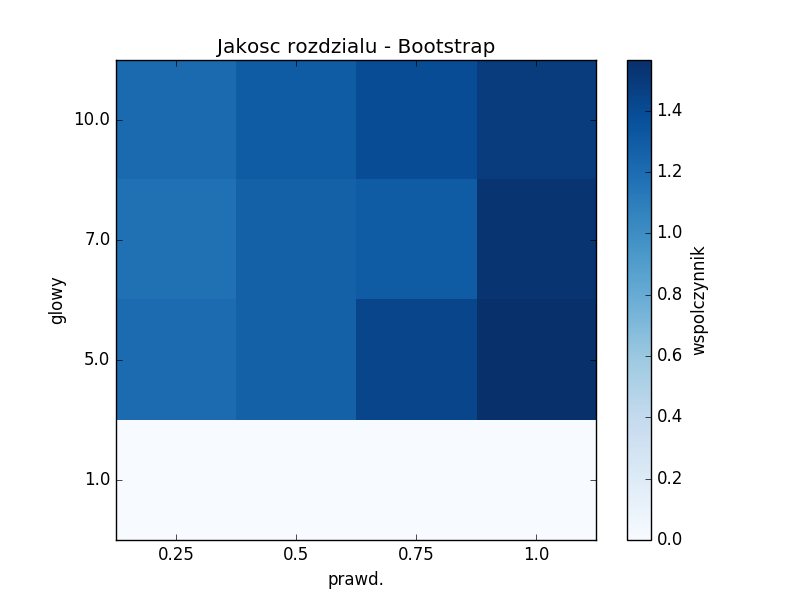
\includegraphics[scale = 0.35]{figures/figures/uncertainties/bootstrap_ratio_mean.png}}{\caption{Bootstrap}\label{fig:b_ratio_mean}}
		\ffigbox{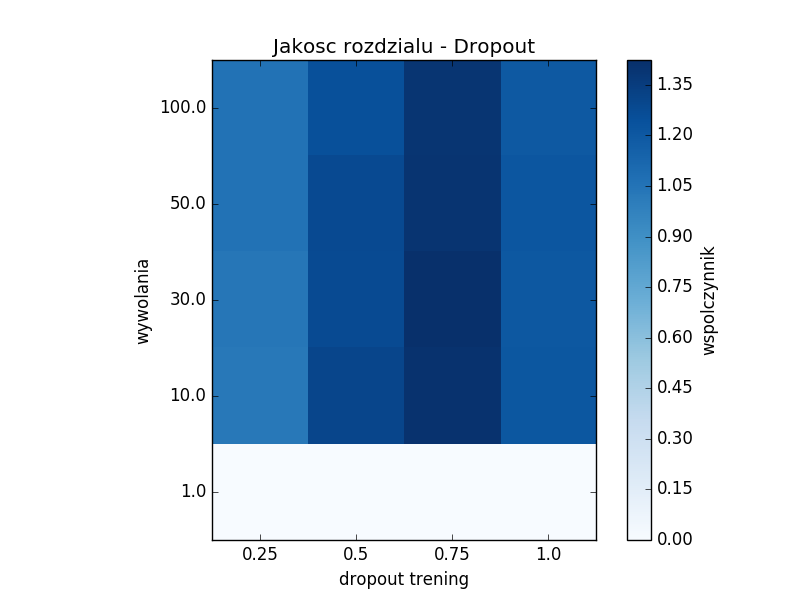
\includegraphics[scale = 0.35]{figures/figures/uncertainties/dropout_ratio_mean.png}}{\caption{Dropout}\label{fig:d_ratio_mean}}
	\end{floatrow}
\end{figure}

\begin{figure}[H]
	\begin{floatrow}
		\ffigbox{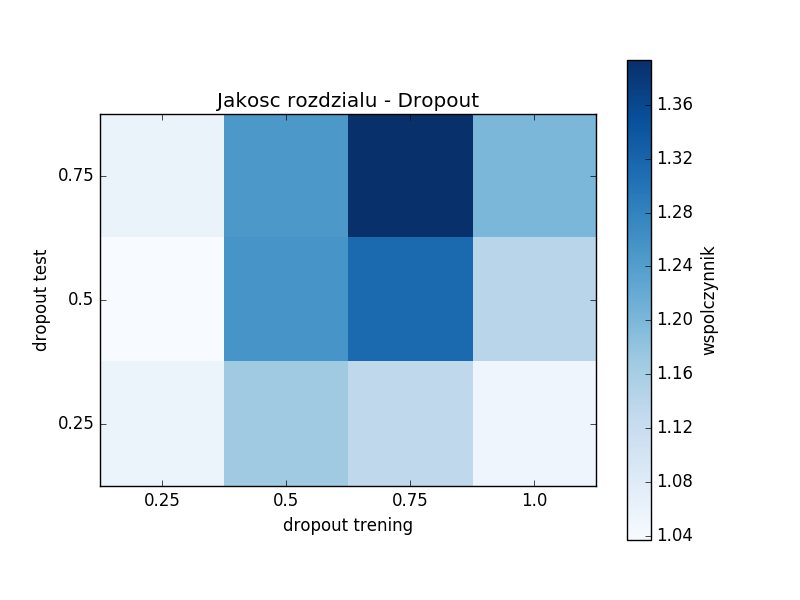
\includegraphics[scale = 0.35]{figures/figures/uncertainties/dropout_ratio_mean2.png}}{\caption{Dropout}\label{fig:d_ratio_mean2}}
		\ffigbox{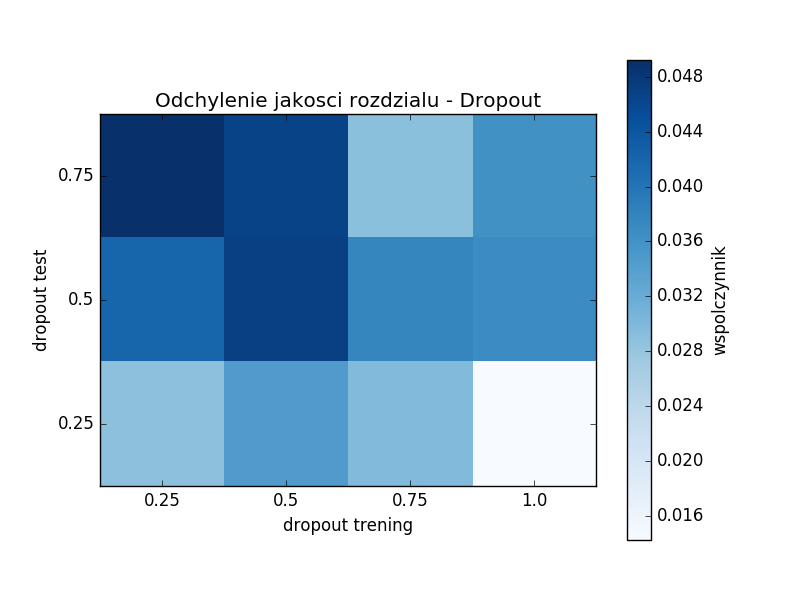
\includegraphics[scale = 0.35]{figures/figures/uncertainties/dropout_ratio_variance2.png}}{\caption{Dropout}\label{fig:d_ratio_var2}}
	\end{floatrow}
\end{figure}

\begin{figure}[H]
	\begin{floatrow}
		\ffigbox{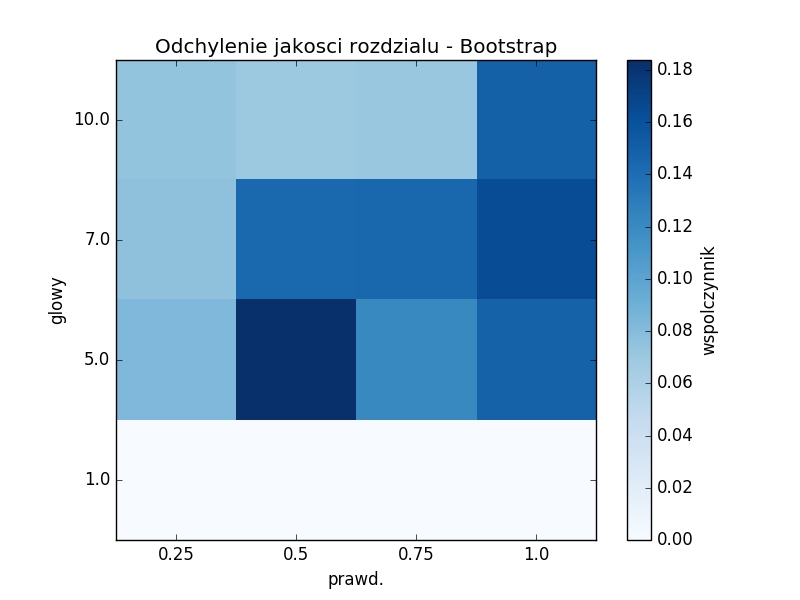
\includegraphics[scale = 0.35]{figures/figures/uncertainties/bootstrap_ratio_variance.png}}{\caption{Bootstrap}\label{fig:b_ratio_var}}
		\ffigbox{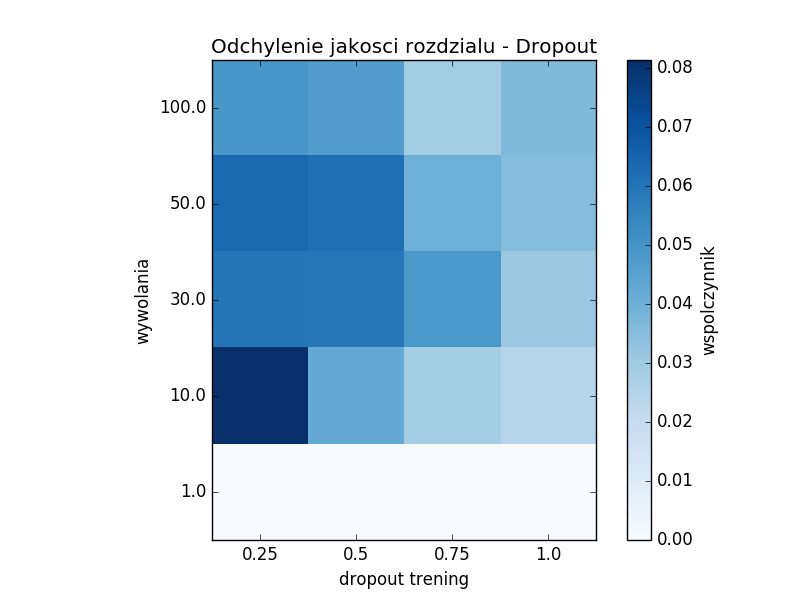
\includegraphics[scale = 0.35]{figures/figures/uncertainties/dropout_ratio_variance.png}}{\caption{Dropout}\label{fig:d_ratio_var}}
	\end{floatrow}
\end{figure}

Na wykresach \ref{fig:b_acc_mean}, \ref{fig:d_acc_mean}, \ref{fig:d_acc_mean2}, \ref{fig:d_acc_var2}, \ref{fig:d_acc_var}, \ref{fig:b_acc_var} przedstawiono średnie i odchylenia standardowe dokładności klasyfikacji uzyskane dla poszczególnych konfiguracji eksperymentów. Wyniki przedstawiają się podobnie jak dla miary $quality_{ND}$. Lepsze wyniki osiąga Bootstrap (44.81\% dla 5 głów i prawdopodobieństwa 0.75, 43.64\%  dla 5 głów i prawdopodobieństwa 1), a jego wyniki są podobne dla wszystkich sensownych parametrów. Wariancja jest minimalna. Wyniki Dropoutu oscylują dookoła 39\% dla wszystkich sensownych parametrów, przy znacznie większej niż Boostrstrap wariancji (2\%). Warto zauważyć, że dla obu metod wyniki są bardzo dodobne dla szerokich zestawów parametrów, i wyraźnie większe niż w przypadku braku bazowego rozwiązania (zaimplementowane w eksperymencie jako Bootstrap z jedną głową, osiągające 37\% dokładności przy 5\% wariancji. Gorszy wynik bazowej wersji wynika z braku odporności na przeuczenie - Bootstrap i Dropout działają jak regularyzatory).


\begin{figure}[H]
	\begin{floatrow}
		\ffigbox{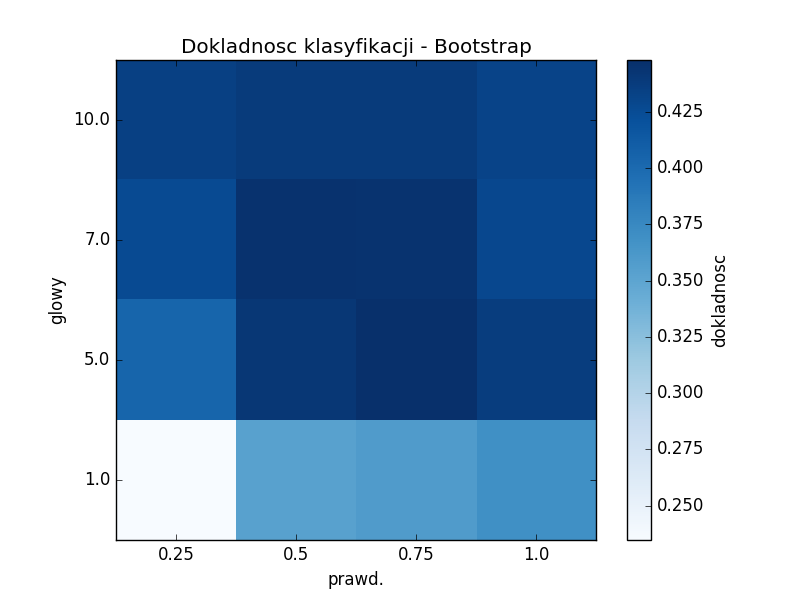
\includegraphics[scale = 0.35]{figures/figures/uncertainties/bootstrap_accuracy_mean.png}}{\caption{Bootstrap}\label{fig:b_acc_mean}}
		\ffigbox{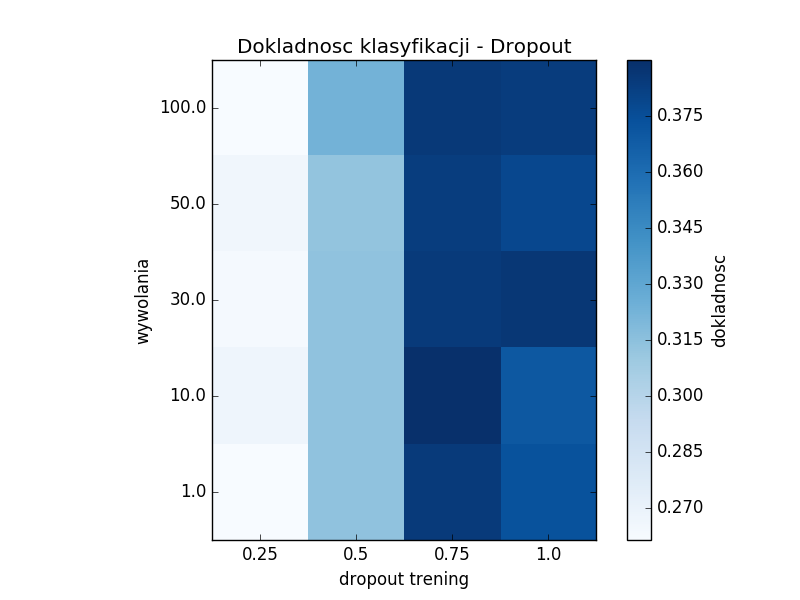
\includegraphics[scale = 0.35]{figures/figures/uncertainties/dropout_accuracy_mean.png}}{\caption{Dropout}\label{fig:d_acc_mean}}
	\end{floatrow}
\end{figure}

\begin{figure}[H]
	\begin{floatrow}
		\ffigbox{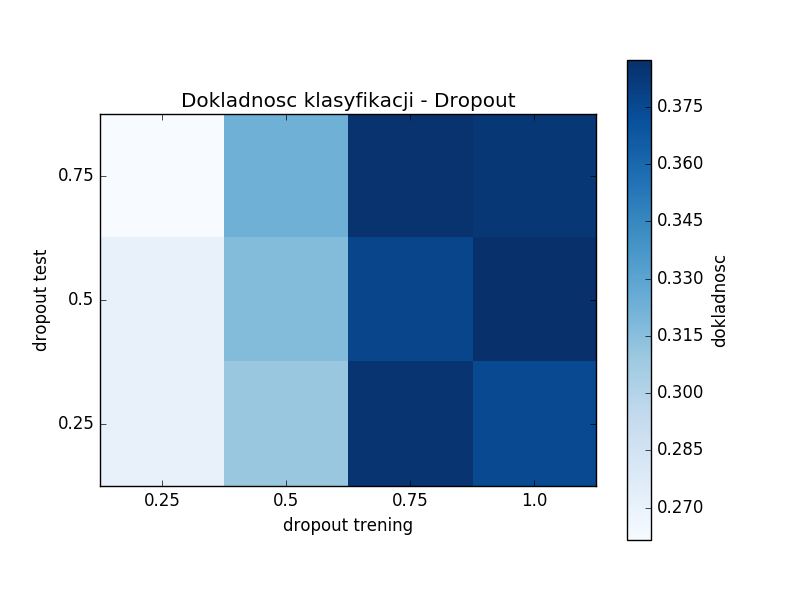
\includegraphics[scale = 0.35]{figures/figures/uncertainties/dropout_accuracy_mean2.png}}{\caption{Dropout}\label{fig:d_acc_mean2}}
		\ffigbox{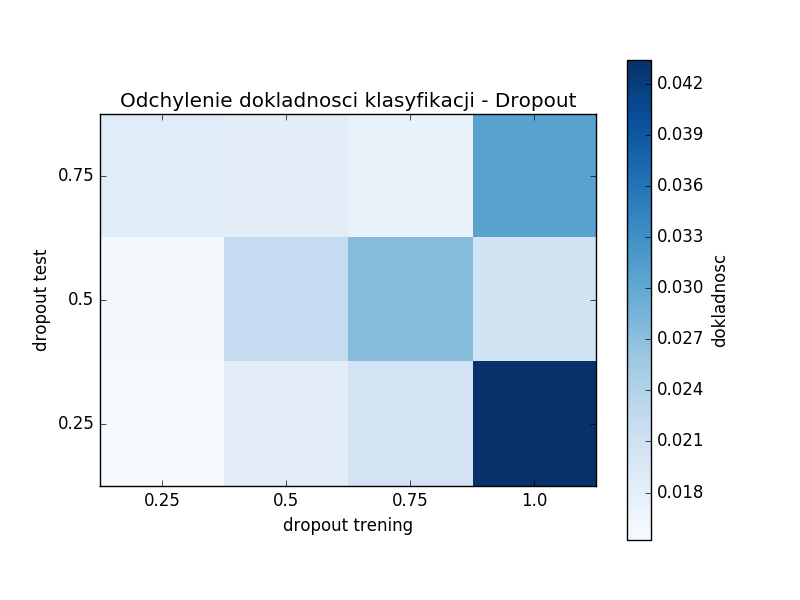
\includegraphics[scale = 0.35]{figures/figures/uncertainties/dropout_accuracy_variance2.png}}{\caption{Dropout}\label{fig:d_acc_var2}}
	\end{floatrow}
\end{figure}

\begin{figure}[H]
	\begin{floatrow}
		\ffigbox{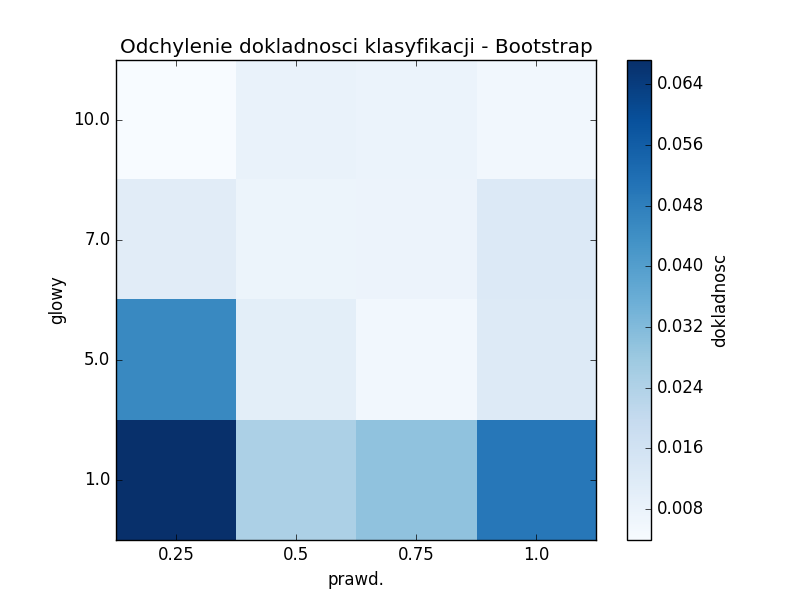
\includegraphics[scale = 0.35]{figures/figures/uncertainties/bootstrap_accuracy_variance.png}}{\caption{Bootstrap}\label{fig:b_acc_var}}
		\ffigbox{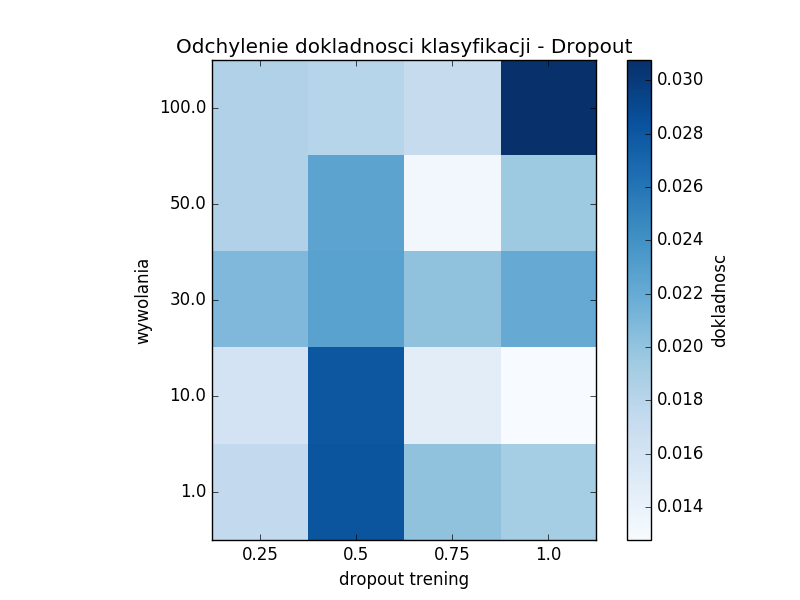
\includegraphics[scale = 0.35]{figures/figures/uncertainties/dropout_accuracy_variance.png}}{\caption{Dropout}\label{fig:d_acc_var}}
	\end{floatrow}
\end{figure}

Na wykresach \ref{fig:b_train_t}, \ref{fig:d_train_t}, \ref{fig:b_test_t}, \ref{fig:d_test_t} przedstawiono czasy treningu i testowania. Na etapie czasu testowania Boostrap wypada znacznie gorzej niż Dropout. 25 sekund dla 5 głów i prawd=0.75 trwa dwa razy dłużej niż 12 sekund osiąganych przez Dropout na wszystkich parametrach, co jest znacznie większym narzutem niż 20\% deklarowane przez autorów metody.

Czas testowania ponownie korzystniejszy jest dla Bootstrapa (0.157s), ponad 5 razy mniej niż Dropout (0.84s). Czas testowania jest bardzo istotny w kontekscie Q-learningu, gdzie dla każdej klatki konieczna jest ocena jakości każdego z możliwych ruchów.

Czas treningu Bootstrapa jest w przybliżeniu liniowo zależny od liczby głów pomnożonych przez prawdopodobieństwo uwzględnienia krotki: $t_{train}  \sim n * p_{incl}$, natomiast czas testu jest w przybliżeniu stały. Czas treningu Dropoutu jest w przybliżeniu stały, natomiast czas testu jest w przybliżeniu liniowo zależny od liczby wywołań $t_{test}  \sim n$.
 
Powody znacznych różnic czasowych mogą tkwić w szczegółach implementacji obu metod. Warto zwrócić uwagę, że dla niektórych zastosowań koszt związany z dodatkowymi obliczeniami może być nieakceptowalny. Natomiast dla zastosowań, dla których koszt działania agenta (czyli koszt zbierania próbek danych) przewyższa koszt działania GPU dłuższy czas działania Bootstrapa może być nieistotny, albo zniwelowany przy wykorzystaniu mocniejszych lub większych zasobów. 

\begin{figure}[H]
	\begin{floatrow}
		\ffigbox{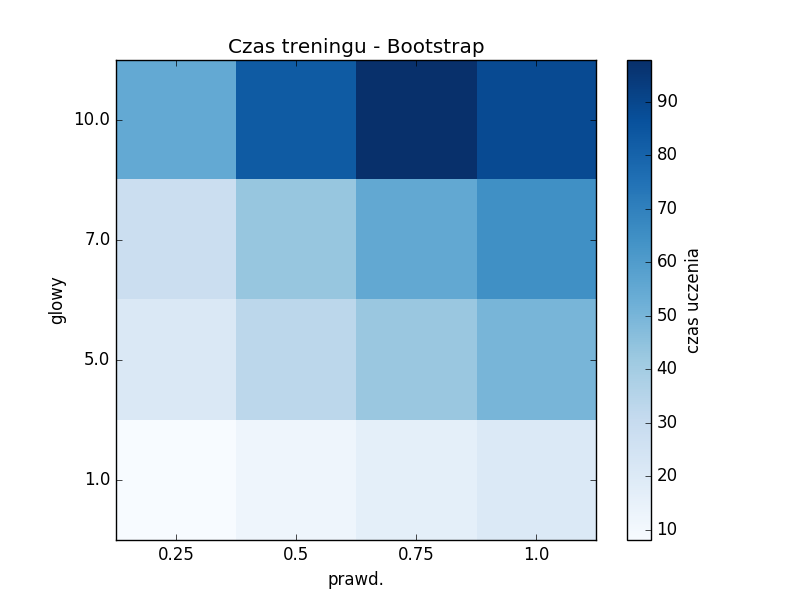
\includegraphics[scale = 0.35]{figures/figures/uncertainties/bootstrap_train_time.png}}{\caption{Dropout}\label{fig:b_train_t}}
		\ffigbox{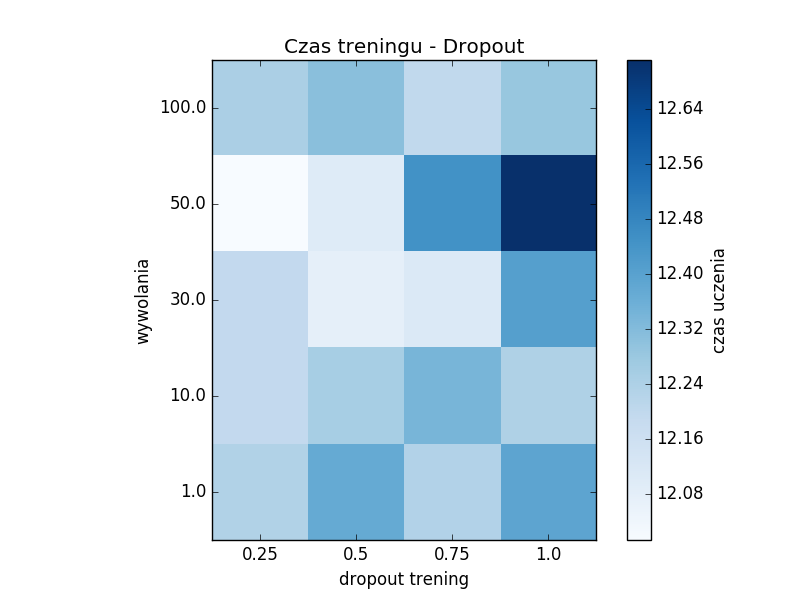
\includegraphics[scale = 0.35]{figures/figures/uncertainties/dropout_train_time.png}}{\caption{Dropout}\label{fig:d_train_t}}
	\end{floatrow}
\end{figure}


\begin{figure}[H]
	\begin{floatrow}
		\ffigbox{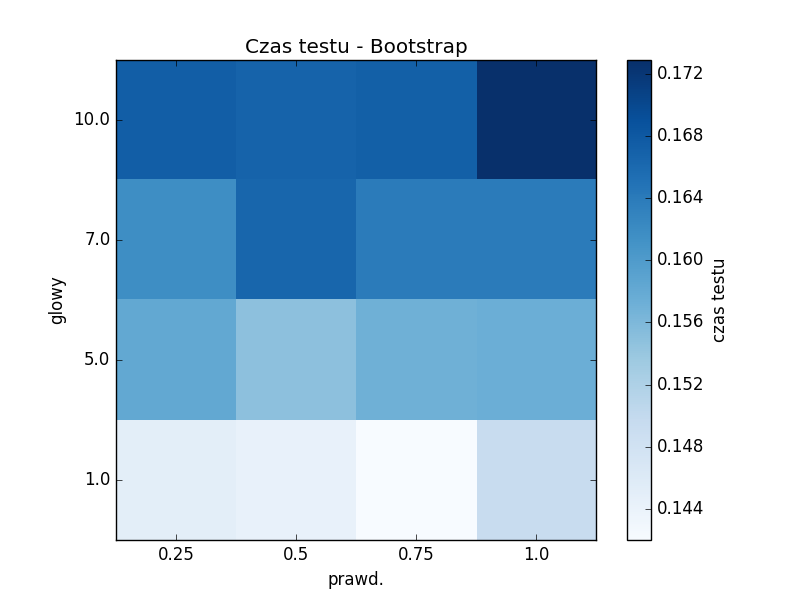
\includegraphics[scale = 0.35]{figures/figures/uncertainties/bootstrap_test_time.png}}{\caption{Dropout}\label{fig:b_test_t}}
		\ffigbox{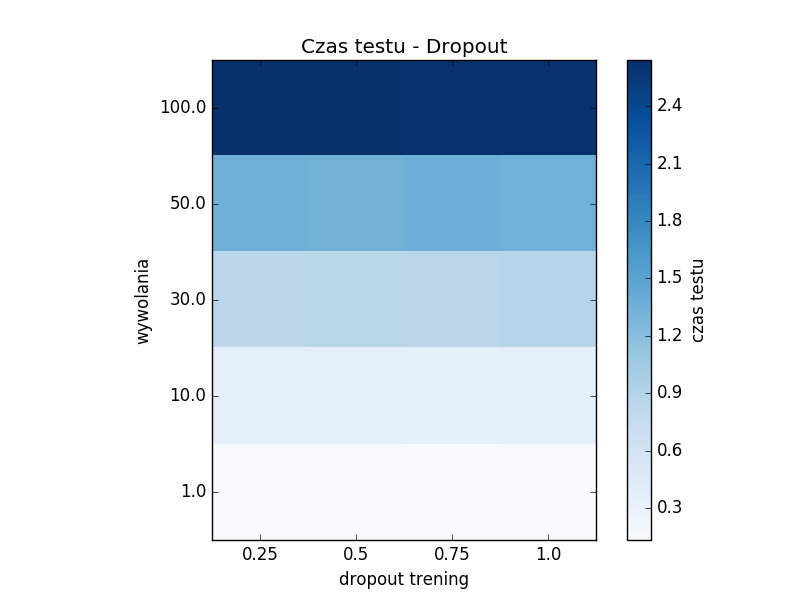
\includegraphics[scale = 0.35]{figures/figures/uncertainties/dropout_test_time.png}}{\caption{Dropout}\label{fig:d_test_t}}
	\end{floatrow}
\end{figure}

Na podstawie przeprowadzonego eksperymentu za najlepszą konfigurację Bootstrapa przyjęto 5 głów i prawdopodobieństwo 0.75, a dla Dropoutu 30 wywołań i oba prawdopodobieństwa równe 0.75

\subsection{Niepewność - wyniki eksperymentu z oceną stopnia pewności}

Dla liczby głów $n=5$ w Bootstrapie i dla liczby wywołań $n=30$ i prawdopodobieństwach dropoutu $p=0.75$ metod współczynnik $quality_{OP}$ dla Bootstrapa z $p=0.75$ wynosi 0.833 przy wariancji 0.11, dla Bootstrapa z $p=1$ wynosi 0.823 przy wariancji 0.10, a dla Dropoutu wynosi 0.925 przy wariancji 0.04. Trafności klasyfikacji dla Bootstrapa z $p=0.75$ wynosi 0.638 a przy wariancji 0.038, dla Bootstrapa z $p=1$ wynosi 0.623 a przy wariancji 0.036 dla Dropoutu wynosi 0.527 przy wariancji 0.032.

\subsection{Niepewność - wnioski}
Bootstrap ma wyraźną przewagę na większości czynników. W drugim eksperymencie jego wyniki są nieznacznie gorsze, ale jako że obie metody osiągają bardzo wysoki współczynnik, ten współczynnik jest pomijalny. Niestety, długi czas treningu Bootstrapa sprawia, że Dropout nie może być kategorycznie odrzucony. Niewykluczone, że w docelowym rozwiązaniu gorsze wyniki Dropoutu będą niezauważalne, natomiast zwiększony czas obliczeń będzie niakceptowalny.

Najważniejszym wnioskiem jest natomiast obserwacja, że obie metody bardzo skutecznie estymują stopień niepewności.


%\chapter{DQN - usprawnienia}
W tym rozdziale przedstawione zostaną pomniejsze zmiany i usprawnienia DQN zbadane w trakcie tworzenia docelowych rozwiązań.

\section{Zapamiętywanie trajektorii}

\section{Eksploracja na bazie niepewności}



%\chapter{Eksperymenty}


% All appendices and extra material, if you have any.
\cleardoublepage\appendix%
%\input{0a-zalacznik.tex}
%\input{0b-pisanie-w-latexu.tex}

% Bibliography (books, articles) starts here.
\bibliographystyle{plalpha}{\raggedright\sloppy\small\bibliography{bibliography}}

% Colophon is a place where you should let others know about copyrights etc.
\ppcolophon

\end{document}
